\section{Задание 3}

\begin{enumerate}
	\item Построить датчик экспоненциального распределения. Проверить для 
    данного распределения свойство отсутствия памяти. Пусть 
    $X_1,X_2,\dots,X_n$~--- независимые экспоненциально распределенные с.в. с 
    параметрами $\lambda_1, \lambda_2, \dots, \lambda_n$ соответственно. Найти 
    распределение случайной величины $Y = \min(X_1, X_2, \dots, X_n)$.
	\item На основе датчика экспоненциального распределения построить датчик 
    пуассоновского распределения.
	\item Построить датчик пуассоновского распределения как предел биномиального
     распределения. С помощью критерия хи-квадрат Пирсона убедиться, что получен
     датчик распределения Пуассона.
	\item Построить датчик стандартного нормального распределения методом 
    моделирования случайных величин парами с переходом в полярные координаты. 
    Проверить при помощи $t$-критерия Стьюдента равенство математических 
    ожиданий, а при помощи критерия Фишера равенство дисперсий.  
\end{enumerate}

\subsection{Экспоненциальное распределение} \label{exp_section}
    Случайная величина $\epsilon$ имеет экспоненциальное распределение с 
    параметром $\lambda$, если ее функция распределения имеет вид
    \begin{equation}
        F(x) = \left\{  \begin{aligned}
            1 - e^{-\lambda x},&\quad x \ge 0,\\
            0,&\quad x < 0.
                        \end{aligned}\right.
    \end{equation}
    Мы будем моделировать $\epsilon \sim \mathrm{Exp}(\lambda)$ с помощью 
    метода обратной функции
    \footnote{см. \cite{NMS} гл. 4 \S 1 ``Метод обратной функции''.},
    согласно которому 
    \[\epsilon \sim -\frac{1}{\lambda} \ln\eta,\]
    где $\eta \sim \mathrm{Uni}\inter{0}{1}$.
    Результат моделирования см. рис. \ref{task3_exp}
    \newpage
    Экспоненциальное распределение обладает свойством отсутствия памяти 
    (рис. \ref{task3_memoexp}), т.е. аналогично \S\,\ref{par12}:
    \[\bigl. \epsilon_m \sim \epsilon ,\quad \forall{m} \in \mathbb{N} \cup \{0\},\]
    где $\epsilon_m := (\gamma \bigr|_{\Omega_m} - m),\: 
    \Omega_m = \epsilon^{-1}(\epsilon \geqslant m) \in \mathcal{A}.$ 
    \bigskip

    \begin{figure}[tbp]
        \centering
        \begin{subfigure}[b]{0.4\textwidth}
            \centering
            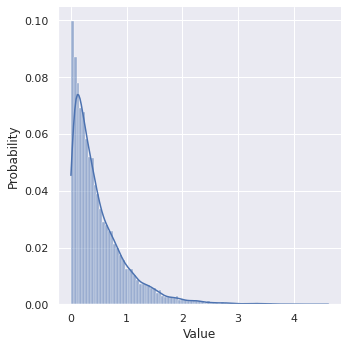
\includegraphics[width=\textwidth]{resources/task3_exp.png}
            \caption{Э.ф.п. экспоненциального распределения}
            \label{task3_exp}
        \end{subfigure}
        \hfill
        \begin{subfigure}[b]{0.5\textwidth}
            \centering
            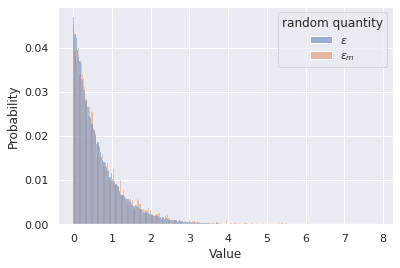
\includegraphics[width=\textwidth]{resources/task3_memoexp.png}
            \caption{Отсутствие памяти ($m = 2$)}
            \label{task3_memoexp}
        \end{subfigure}
        \caption{}
    \end{figure}

    Распределение сл.в. $Y = \min(X_1,X_2,\ldots X_n)$ имеет функцию 
    распределения 
    \begin{multline*}
        F(y) = \Prb{Y < y} = 1 - \Prb{Y \ge 1} = 
        1 - \Prb{\min(X_1,X_2,\ldots X_n) \ge 1} = \\
        1 - \Prb{X_1 \ge y, \ldots, X_n \ge y} = 
        \text{\{в силу независимости сл.в. $X_i$\} } = 
        1 - \prod_{i=1}^{n} \Prb{X_i \ge y} = \\
        1 - \prod_{i=1}^{n} (1 - F_{Exp(\lambda_i)}) = 
        1 - \prod_{i=1}^{n} (1 - (1 - e^{-\lambda_i y})) =
        1 - \prod_{i=1}^{n} e^{-\lambda_i y} = 
        1 - e^{-(\sum_{i=1}^{n} \lambda_i) y}.
    \end{multline*}
    Таким образом
    \[Y \sim \mathrm{Exp}(\sum_{i=1}^{n} \lambda_i)\]
    Cравните результаты, посчитанные для обоих представлений $Y$ 
    на рис. \ref{task3_minexp}.

    \begin{figure}[tbp]
        \centering
        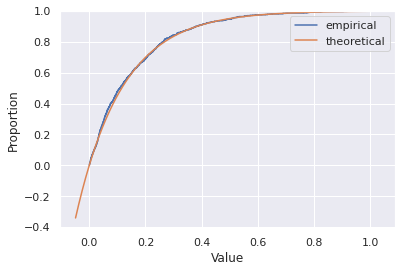
\includegraphics[width=0.7\textwidth]{resources/task3_minexp.png}
        \caption{Э.ф.р. $\mathrm{Exp}(\lambda)$}
        \label{task3_minexp}
    \end{figure}

\subsection{Датчик пуассоновского распределения 1}
    Случайная величина $\pi$ имеет распределение Пуассона с параметром 
    $\lambda > 0$, если $\Prb{\pi = k} = \dfrac{\lambda^k}{k!} e^{-\lambda}$.
    Для $\pi \sim \mathrm{Pois}(\lambda)$ верно следующее представление
    \footnote{см. \cite{NMS} гл. 5 \S 1 ``Моделирование дискретных величин''.}
    \[\pi = \max_{\mathbb{N}\cup\{0\}}(n \mid S_n = \sum_{i=1}^{n} \epsilon_i \le 1),\]
    где $\epsilon_1,\epsilon_2,\ldots$~--- экспоненциальные с параметром $\lambda$ 
    н.о.р.с.в. 

    Результат моделировния см. рис. \ref{task3_pois1}

\subsection{Датчик пуассоновского распределения 2}
    Известно, что распределение $\mathrm{Pois}(\lambda)$ получается из 
    биномиального $\mathrm{Bin}(n,p)$ предельным переходом при $n\rightarrow 
    \infty$, $p \rightarrow 0$, $np \rightarrow \lambda$. Результат моделирования 
    распределения пуассона на основе этого приниципа предоставлен на рис. \ref{task3_pois2}.

    \begin{figure}[tbp]
        \centering
        \begin{subfigure}[b]{0.48\textwidth}
            \centering
            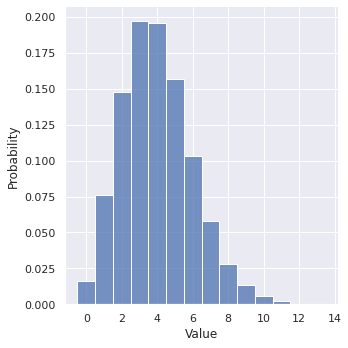
\includegraphics[width=\textwidth]{resources/task3_pois1.png}
            \caption{}
            \label{task3_pois1}
        \end{subfigure}
        \hfill
        \begin{subfigure}[b]{0.48\textwidth}
            \centering
            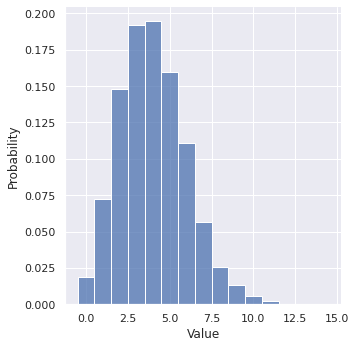
\includegraphics[width=\textwidth]{resources/task3_pois2.png}
            \caption{}
            \label{task3_pois2}
        \end{subfigure}
        \caption{Гистограммы датчиков распределения Пуассона}
    \end{figure}

    Проверим корректность нашего датчика при помощи критерия хи-квадрат Пирсона.

    Пусть $X_1,\ldots X_n$~--- выборка. Разобьем множество значений $\xi_1$ на 
    $N$ промежутков (возможно, бесконечных) $\Delta_j = (a_j, b_j], 
    j = 1,\ldots N.$ Положим $p_j = \Prb{X_1 \in \Delta_j}$, а случайные 
    величины $\nu_j$~--- равными количеству элементов выборки в $\Delta_j$.
    
    \newpage
    Так, статистикой критерия Пирсона служит величина 
    \begin{equation}
        X_n^2 = \sum\limits_{j=1}^N \dfrac{(\nu_j - n p_j)^2}{p_j},
    \end{equation}
    предел которой, при $n\rightarrow \infty$ имеет распределение $\chi_{N-1}^2$.

    Поскольку распределение Пуассона дискретно, промежутки $\Delta_j$ зададим 
    как $\Delta_j = \{j-1\}, j = 1,\ldots, N-1;\quad 
    \Delta_N = \{j\in \mathbb{N}: j > N-1\}$. $N$ положим равным приблизительно 
    $\log_2 n$. Теперь вычислим соответствующие частоты, вероятности и 
    статистику. По результатам вычислений гипотеза о корректности принимается с 
    уровнем значимости 5\%.

\subsection{Датчик стандартного нормального распределения 1} \label{3.4}
    Нормальное распределение~--- абсолютно непрерывное распределение с 
    плотностью $p(x) = \frac{1}{\sigma \sqrt{2\pi}} 
    e^{-\frac{1}{2}(\frac{x-\mu}{\sigma})^2}$, где параметры $\mu, \sigma$~--- 
    математическое ожидание и среднеквадратическое отклонение соответственно.

    С помощью нелинейного преобразования пары н.о.р.с.в. $\eta_1, \eta_2 \sim 
    \mathrm{U}\segm{0}{1}$ можно получить две н.о.р.с.в. $X,Y \sim \mathcal{N}(0,1)$:
    \begin{gather*}
        X = -\sqrt{-2\ln\eta_1}\cos(2\pi\eta_2),\\  
        Y = -\sqrt{-2\ln\eta_1}\sin(2\pi\eta_2). 
    \end{gather*}
    Результат cмоделированной таким способом стандартной нормальной случайной 
    величины см. \ref{task3_norm}.

    \begin{figure}[tbp]
        \centering
        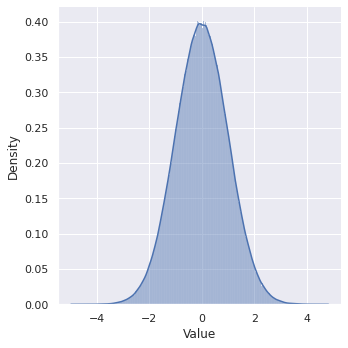
\includegraphics[width=0.5\textwidth]{resources/task3_norm.png}
        \caption{Э.ф.п. нормального распредления}
        \label{task3_norm}
    \end{figure}


    Для проверки однородности двух независимых нормальных выборок (в нашем 
    случае это $X$ и $Y$) используют критерии Фишера и Стьюдента. Оба критерия 
    имеют двустороннюю критическую области, т.о. при заданном уровне значимости 
    $\alpha$ нулевая гипотеза принимается в случае если статистика приняла 
    значение между $(\alpha/2)$ и $(1-\alpha/2)$ квантилями соответствующего 
    распределения.

    Критерий Фишера служит для проверки гипотезы о соответствии дисперсий 
    двух распределений. Его статистика имеет вид
    \begin{equation}\label{Fischer}
        \dfrac{S_1^2}{S_2^2} = \dfrac{\frac{1}{n-1}\sum_{i=1}^n (X_i-\overline X)^2}
        {\frac{1}{m-1}\sum_{j=1}^m (Y_j-\overline Y)^2},
    \end{equation}
    и распределена по закону $F_{n-1,m-1}$, т.е так же как и случайная величина 
    $\zeta~=~(\frac{1}{n-1}\xi)/(\frac{1}{m-1}\eta)$, где $\xi \sim \chi_{n-1}^2,
    \eta \sim \chi_{m-1}^2$, $\xi$ и $\eta$ независимы.
    
    В результате вычисления статистики \eqref{Fischer} гипотеза о соответствии 
    дисперсий принимается с уровнем значимости $\alpha = 5\%$.

    Критерий Стьюдента позволяет проверить гипотезу о соответствии математических
    ожиданий. Статистика в данном случае имеет вид
    \begin{equation}
        \frac{\sqrt{\frac{nm}{n+m}}(\overline X - \overline Y) (n+m-2)} 
        {[(n-1)S_1^2 + (m-1)S_2^2]} \sim t_{n+m-2},
    \end{equation}
    где $t_{n+m-2}$~--- распределение Стьюдента с $(n+m-2)$ степенями свободы.

    Значение статистики Стьюдента позволяет нам принять гипотезу о равенстве 
    мат. ожиданий с уровнем значимости $\alpha = 5\%$, что, в совокупности с уже
    установленным равенством дисперсий дает нам сделать вывод об 
    однородности нормальных выборок $X$ и $Y$ с тем же уровнем значимости.

